\section{Experimentos realizados y resultados obtenidos}
\subsection{Experimentos con el Perceptrón}
\label{subsec:perceptronexperiment}

El primer experimento que hemos realizado con el perceptrón ha sido sencillo, con el objetivo de comprobar que el funcionamiento era el esperado y, sobre todo, ver gráficamente como el PLA iba evolucionando los pesos y cual iba siendo la evolución. La función que hemos intentado aproximar con el perceptrón ha sido la función AND, la cual se describe en el algoritmo \ref{alg:andfunction}.

\begin{algorithm}
    
    \eIf{$a * b == 1$}
    {
        $return$ 1$;$
    }
    {
        $return$ 0$;$
    }

	\caption{Función AND}
	\label{alg:andfunction}
\end{algorithm}

La función AND es linealmente separable, por lo que el perceptrón debería de poder separar los puntos eventualmente. En la figura \ref{fig:andFunctionTargets} se muestran los puntos que queremos separar (como subindice tienen el valor que se espera por el perceptrón).

\begin{figure}[H]
	\centering
	\includegraphics[width=1\textwidth]{{"Figures/Perceptrón. Targets"}.png}
	\caption{Puntos de la función AND}
	\label{fig:andFunctionTargets}
\end{figure}

\begin{figure}[H]
    \begin{tabular}{cc}
      \includegraphics[width=65mm\textwidth]{{"Figures/Perceptrón. PLA - 1st iteration"}.png} &  \includegraphics[width=65mm\textwidth]{{"Figures/Perceptrón. PLA - 2nd iteration"}.png} \\
    1a iteración PLA (25\% acierto) & 2a iteración PLA (75\% acierto) \\[6pt]
     \includegraphics[width=65mm\textwidth]{{"Figures/Perceptrón. PLA - 3rd iteration"}.png} &   \includegraphics[width=65mm\textwidth]{{"Figures/Perceptrón. PLA - 4th iteration"}.png} \\
    3a iteración PLA (75\% acierto) & 4a iteración PLA (50\% acierto) \\[6pt]
    \includegraphics[width=65mm\textwidth]{{"Figures/Perceptrón. PLA - 5th iteration"}.png} &   \includegraphics[width=65mm\textwidth]{{"Figures/Perceptrón. PLA - 6th iteration"}.png} \\
    5a iteración PLA (75\% acierto) & 6a iteración PLA (50\% acierto) \\[6pt]
    \multicolumn{2}{c}{\includegraphics[width=65mm\textwidth]{{"Figures/Perceptrón. PLA - 7th iteration"}.png} }\\
    \multicolumn{2}{c}{7a iteración PLA (100\% acierto)}
    \end{tabular}
\caption{Iteraciones del PLA para la función AND}
\label{fig:andFunctionPLAIterations}
\end{figure}

\newpage

En la figura \ref{fig:andFunctionPLAIterations} podemos ver como el PLA ha ido ajustando los pesos para buscar el plano que separa correctamente estos puntos.

Una vez observamos los resultados nos damos cuenta de algo, y es que al aplicar la función signo hay una recta que corta con el plano XY, y por lo tanto podemos reducir los resultados en 1 dimensión y dejar los datos mucho más claros (pasar los resultados de las 3 dimensiones al plano XY en 2 dimensiones). Lo que hay que hacer para esto es igualar la ecuación obtenida del plano (no es encesario que sea con la función signo aplicada) y resolver el sistema de ecuaciones que se forma con el plano XY.

\[PlanoXY: (x,y,z)=(x,y,0)\equiv z=0\]
\[PlanoFunciónAND:z=1.35065*x+0.657562*y-1.35867\]

Al resolver estas ecuaciones nos queda la siguiente ecuación:

\[y=-\dfrac{1.35065}{0.657562}*x+\dfrac{1.35867}{0.657562}\]

La ecuación anterior es el resultado de la intersección, que se puede observar en la figura \ref{fig:andFunctionPLAIterations} (7a iteración), con el plano XY. El resultado lo podemos observar en la figura \ref{plot:perceptronANDFunction2dim}.

\begin{figure}[!h]
\centering
    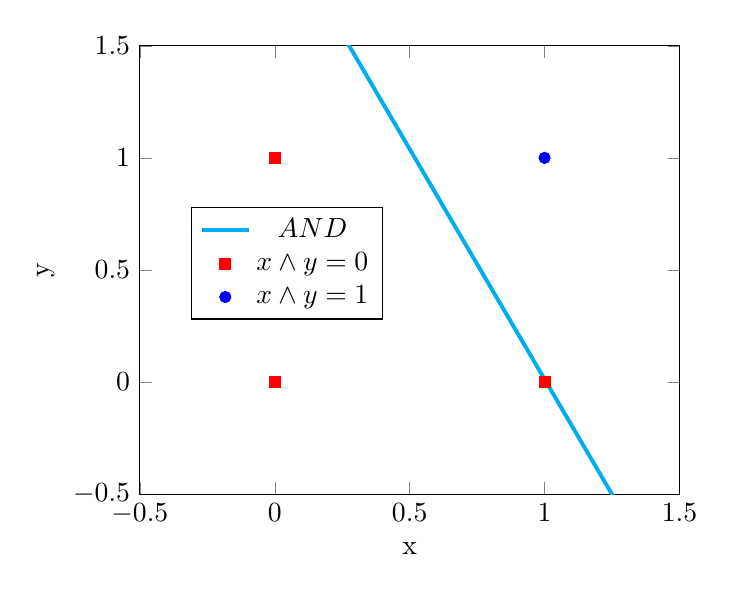
\begin{tikzpicture}
    \begin{axis}[ xlabel=x, ylabel=y,xmin=-0.5,xmax=1.5,ymin=-0.5,ymax=1.5,legend style={at={(0.45,0.64)}}]
    
        \addplot[color=cyan,mark=none,samples=2,line width=0.5mm]{-(1.35065/0.657562)*x+(1.35867/0.657562)};
        \addlegendentry{$AND$}
    
        \addplot [only marks,color=red,mark=square*] table {
            0 0
            0 1
            1 0
        };
        \addlegendentry{$x\wedge y = 0$}
        
        \addplot [only marks,color=blue,mark=*] table {
            1 1
        };
        \addlegendentry{$x\wedge y = 1$}

    
    \end{axis}
    \end{tikzpicture}
\caption{Ecuación resultante de la función AND}
\label{plot:perceptronANDFunction2dim}
\end{figure}

\newpage
Algo interesante que podemos observar con este experimento es que el porcentaje de acierto no siempre aumenta (la razón ya se explicó en la sección \ref{subsec:perceptron}), por lo que si en este experimento hubiéramos configurado un número de épocas igual a 5 habríamos obtenido como resultado final un 50\% de aciertos, no un 75\%, en el caso de que no hubiéramos implementado el algoritmo del \textit{Pocket}.

\begin{figure}[!h]
\centering
    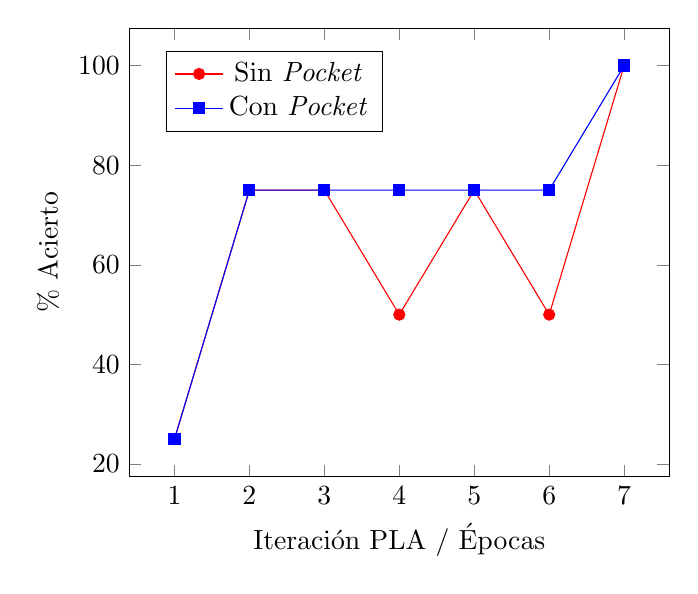
\begin{tikzpicture}
    \begin{axis}[ xlabel=Iteración PLA / Épocas, ylabel=\% Acierto, legend style={at={(0.47,0.95)}}]
        
        \addplot[color=red,mark=*] coordinates
        {
        (1,25)
        (2,75)
        (3,75)
        (4,50)
        (5,75)
        (6,50)
        (7,100)
        };
        \addlegendentry{Sin \textit{Pocket}}
        
        \addplot[color=blue,mark=square*] coordinates
        {
        (1,25)
        (2,75)
        (3,75)
        (4,75)
        (5,75)
        (6,75)
        (7,100)
        };
        \addlegendentry{Con \textit{Pocket}}
    \end{axis}
    \end{tikzpicture}
\caption{Resultados del PLA con y sin \textit{Pocket}}
\label{plot:perceptronResultsWithAndWithoutPocket}
\end{figure}

Como ya hemos comentado, el algoritmo del \textit{Pocket} también podemos verle la utilidad en este sencillo experimento. En la figura \ref{plot:perceptronResultsWithAndWithoutPocket} se ve como a cada iteración que se ejecuta del PLA (también se puede ver como una época) dependiendo de si tenemos el algoritmo del \textit{Pocket} o no, al final obtendremos un resultado u otro. Esto es esencial cuando nos enfrentamos a un problema que no es linealmente separable y la mayoría de los problemas a los que se les puede aplicar el perceptrón y obtener unos resultados aceptables no serán linealmente separables.

\newpage
Finalmente, hemos realizado 3 experimentos más, donde cada experimento intenta aproximar una función diferente. Las funciones que intentan aproximar son las siguientes;

\[y=0.5\]
\[y=0.5*x\]
\[y=-0.5*x+0.5\]

Los resultados han sido muy favorables ya que con pocas épocas hemos conseguido una muy buena aproximación, como podemos ver en las figuras \ref{fig:perceptronFunction2Experiment}, \ref{fig:perceptronFunction3Experiment} y \ref{fig:perceptronFunction4Experiment}. En los todos los experimentos realizados se consiguió el 100\% de aciertos. Además, en las figuras también está la función que intentaba aproximar y en color rojo marcado el error cometido.

\begin{figure}[H]
    \centering
    
    \begin{tikzpicture}
    \begin{axis}[width=12cm,xlabel=x, ylabel=y, legend style={at={(0.95,0.95)}},xmin=0,xmax=1]
    
        \addplot table [only marks,x=x, y=y, col sep=comma,color=red] {CSVFiles/function2_+1.csv};
        \addlegendentry{Valores \textgreater 0.5}
        
        \addplot table [only marks,x=x, y=y, col sep=comma,color=blue] {CSVFiles/function2_-1.csv};
        \addlegendentry{Valores \textless 0.5};
        
        \addplot[name path=A,color=cyan,mark=none,samples=2,line width=0.5mm]{(0.130447/5.34289)*x+(2.51017/5.34289)};
        \addlegendentry{Perceptrón};
        
        \addplot[name path=B,color=magenta,mark=none,samples=2,line width=0.5mm]{0.5};
        \addlegendentry{y=0.5};
        
        \addplot[pattern=north west lines, pattern color=red!90]fill between[of=A and B, soft clip={domain=0:1}];
    
    \end{axis}
    \end{tikzpicture}
    
    \caption{Función $y=0.5$}
    \label{fig:perceptronFunction2Experiment}
\end{figure}

\begin{figure}[H]
    \centering
    
    \begin{tikzpicture}
    \begin{axis}[width=12cm,xlabel=x, ylabel=y, legend style={at={(0.95,0.95)}},xmin=0,xmax=1]
    
        \addplot table [only marks,x=x, y=y, col sep=comma,color=red] {CSVFiles/function3_+1.csv};
        \addlegendentry{Valores \textgreater 0.5*x}
        
        \addplot table [only marks,x=x, y=y, col sep=comma,color=blue] {CSVFiles/function3_-1.csv};
        \addlegendentry{Valores \textless 0.5*x};
        
        \addplot[name path=A,color=cyan,mark=none,samples=2,line width=0.5mm]{(2.20144/7.48173)*x+(0.897836/7.48173)};
        \addlegendentry{Perceptrón};
        
        \addplot[name path=B,color=magenta,mark=none,samples=2,line width=0.5mm]{0.5*x};
        \addlegendentry{y=0.5*x};
        
        \addplot[pattern=north west lines, pattern color=red!90]fill between[of=A and B, soft clip={domain=0:1}];
    
    \end{axis}
    \end{tikzpicture}
    
    \caption{Función $y=0.5*x$}
    \label{fig:perceptronFunction3Experiment}
\end{figure}

\begin{figure}[H]
    \centering
    
    \begin{tikzpicture}
    \begin{axis}[width=12cm,xlabel=x, ylabel=y, legend style={at={(0.95,0.95)}},xmin=0,xmax=1]
    
        \addplot table [only marks,x=x, y=y, col sep=comma,color=red] {CSVFiles/function4_+1.csv};
        \addlegendentry{Valores \textgreater -0.5*x+0.5}
        
        \addplot table [only marks,x=x, y=y, col sep=comma,color=blue] {CSVFiles/function4_-1.csv};
        \addlegendentry{Valores \textless -0.5*x+0.5};
        
        \addplot[name path=A,color=cyan,mark=none,samples=2,line width=0.5mm]{-(1.79482/3.08686)*x+(1.78977/3.08686)};
        \addlegendentry{Perceptrón};
        
        \addplot[name path=B,color=magenta,mark=none,samples=2,line width=0.5mm]{-0.5*x+0.5};
        \addlegendentry{y=-0.5*x+0.5};
        
        \addplot[pattern=north west lines, pattern color=red!90]fill between[of=A and B, soft clip={domain=0:1}];
    
    \end{axis}
    \end{tikzpicture}
    
    \caption{Función $y=-0.5*x+0.5$}
    \label{fig:perceptronFunction4Experiment}
\end{figure}

Hemos realizado un último experimento donde el objetivo es ver la limitación del perceptrón. Como se comentó en la sección \ref{subsec:perceptron}, el perceptrón nos asegura que convergerá, eventualmente, si los datos son linealmente separables, pero no nos asegura que convergerá si no lo son y de echo no converge en su totalidad, pero aún puede darnos buenos resultados e incluso podríamos recurrir a las transformaciones no lineales para convertir los datos que no son linealmente separables en linealmente separables.

El experimento trata de aproximar la función

\[y=\dfrac{1}{10*x}\]

la cual no es lineal. El resultado se puede observar en la figura \ref{fig:perceptronFunction5Experiment}, donde el acierto ha sido de un 88\%.

\begin{figure}[H]
    \centering
    
    \begin{tikzpicture}
    \begin{axis}[width=12cm,xlabel=x, ylabel=y, legend style={at={(0.95,0.95)}},xmin=0,xmax=1,ymin=0,ymax=1]
    
        \addplot table [only marks,x=x, y=y, col sep=comma,color=red] {CSVFiles/function5_+1.csv};
        \addlegendentry{Valores \textgreater 1/(10*x)};
        
        \addplot table [only marks,x=x, y=y, col sep=comma,color=blue] {CSVFiles/function5_-1.csv};
        \addlegendentry{Valores \textless 1/(10*x)};
        
        \addplot[name path=A,color=cyan,mark=none,samples=2,line width=0.5mm]{-(1.91923/4.17328)*x+(1.94614/4.17328)};
        \addlegendentry{Perceptrón};
        
        \addplot[name path=B,color=magenta,mark=none,samples=40,line width=0.5mm,domain=0.1:1]{1/(10*x)};
        \addlegendentry{1/(10*x)};
        
        \addplot [name path=C,domain=0:0.1] {1};
        
        \addplot[pattern=north west lines, pattern color=red!90]fill between[of=A and B, soft clip={domain=0.1:1}];
        
        \addplot[pattern=north west lines, pattern color=red!90]fill between[of=A and C, soft clip={domain=0:0.1}];
        
    
    \end{axis}
    \end{tikzpicture}
    
    \caption{Función $y=\dfrac{1}{10*x}$}
    \label{fig:perceptronFunction5Experiment}
\end{figure}

En el último experimento de la figura \ref{fig:perceptronFunction5Experiment} utilizamos 200 puntos en vez de los 40 que hemos utilizado en los otros experimentos para que el patrón de la función se notara más visualmente y con el objetivo de que hubieran más puntos que el perceptrón no pudiera aproximar.

\newpage
\subsection{Experimentos con la Red Neuronal}
\label{subsec:nnexperiments}

\newpage
\subsection{Experimentos con la Red Neuronal: \textit{Dropout}}
\label{subsubsec:nnexperiments:Dropout}

\newpage
\subsection{Experimentos con la Red Neuronal: \textit{Cross Validation} 10}
\label{subsubsec:nnexperiments:CV10}

\newpage
\subsection{Experimentos con la Red Neuronal y Genético: \textit{GANN}}
\label{subsubsec:nnexperiments:GANN}

Los experimentos realizados con el GANN han consistido en la variación de diferentes parámetros como pueden ser la activación del elitismo, cambiar la probabilidad de mutación, etc. y ver como se convergía antes, o como se alcanzaban mejores puntuaciones, etc.

El primer experimento vamos a ver los mejores resultados obtenidos en el videojuego Breakout cuando tenemos elitismo y cuando no lo tenemos. Como podemos observar en la figura \ref{fig:breakoutWithAndWithoutElitism}, el elitismo hace que no perdamos el mejor individuo de una generación, como sí que sucede cuando no lo utilizamos. El elitismo es parecido al algoritmo del \textit{Pocket} que vimos en la sección \ref{subsec:perceptron} con la teoría y en la sección \ref{subsec:perceptronexperiment} con los experimentos.

\begin{figure}[!h]
    \centering
    
    \begin{tikzpicture}
    \begin{axis}[width=12cm,xlabel=Generaciones, ylabel=Puntuación, legend style={at={(0.95,0.18)}}]
    
        \addplot table [x=Generation, y=ScoreElitism0, col sep=comma] {CSVFiles/experiment1breakout100generations500population1factorWeights.csv};
        \addlegendentry{Elitismo = 0}
        
        \addplot table [x=Generation, y=ScoreElitism5, col sep=comma] {CSVFiles/experiment1breakout100generations500population1factorWeights.csv};
        \addlegendentry{Elitismo = 5}
    
    \end{axis}
    \end{tikzpicture}
    
    \caption{Breakout con y sin Elitismo}
    \label{fig:breakoutWithAndWithoutElitism}
\end{figure}

Otro de los experimentos que realizamos fue inicializar los pesos en el rango [-2.0, 2.0] en vez de [-1.0, 1.0]. Este cambio depende mucho del problema, ya que al aumentar el rango al doble de posibles valores debería de ser más dificil de obtener una mejor inicialización, pero eventualmente, como ahora tenemos pesos que no están solo limitados al rango [-1.0, 1.0] sino que ahora pueden tener un rango mayor de valores, puede que ahora tengan la posibilidad de obtener mejores resultados que antes. Esto es justo lo que sucede en la figura \ref{fig:breakoutWeightsFactor2}. Hay que destacar que en ambos hay un elitismo de 5 y el resto de parámetros son iguales para poder comparar los resultados. Lo único que cambia es el factor por el que se multiplica el rango de los números reales. El resultado al final es que converge a una puntuación mayor a pesar de tener que buscar unos pesos y \textit{biases} en un rango de valores más amplios, por lo que quizá en tener ese rango de valores le ha permitido aprender mejor a como jugar.

\begin{figure}[!h]
    \centering
    
    \begin{tikzpicture}
    \begin{axis}[width=12cm,xlabel=Generaciones, ylabel=Puntuación, legend style={at={(0.95,0.18)}}]
    
        \addplot table [x=Generation, y=WeightsFactor1, col sep=comma] {CSVFiles/experiment2breakout100generations500population5elitism.csv};
        \addlegendentry{Rango = [-1.0, 1.0]}
        
        \addplot table [x=Generation, y=WeightsFactor2, col sep=comma] {CSVFiles/experiment2breakout100generations500population5elitism.csv};
        \addlegendentry{Rango = [-2.0, 2.0]}
    
    \end{axis}
    \end{tikzpicture}
    
    \caption{Breakout con diferente rango de valores reales}
    \label{fig:breakoutWeightsFactor2}
\end{figure}

Una vez tenemos muchos individuos que han jugado bien al videojuego podemos plantearnos lo que ya se comentó en la sección \ref{subsubsec:nn:gann}, en la que se habló de la inicialización con una distribución de probabilidad. El modo en el que nosotros hemos realizado este experimento es cogiendo los 10 pesos de los 7 mejores individuos que hemos encontrado, y hemos unido los puntos para comprobar si se seguía un patrón en los pesos, algo que pudiéramos utilizar como distribución de probabilidad. En la figura \ref{fig:breakoutProbabilityDistribution} podemos ver que los 10 pesos de los mejores individuos claramente siguen un patrón: la mayoría están próximos y en casi todos los casos se cumple que yendo de un punto a otro, o todos tienen pendiente ascendente o todos tienen pendiente descendente.

\begin{figure}[!h]
    \centering
    
    \begin{tikzpicture}
    \begin{axis}[width=11cm,xlabel=Índice del peso, ylabel=Valor del peso, legend style={at={(1.1,1.1)}}]
    
        \addplot table [x=Weight, y=b822, col sep=comma] {CSVFiles/breakoutProbabilityDistribution.csv};
        \addlegendentry{Puntuación = 822}
        
        \addplot table [x=Weight, y=b833, col sep=comma] {CSVFiles/breakoutProbabilityDistribution.csv};
        \addlegendentry{Puntuación = 833}
        
        \addplot table [x=Weight, y=b847, col sep=comma] {CSVFiles/breakoutProbabilityDistribution.csv};
        \addlegendentry{Puntuación = 847}
        
        \addplot table [x=Weight, y=b860a1, col sep=comma] {CSVFiles/breakoutProbabilityDistribution.csv};
        \addlegendentry{Puntuación = 860}
        
        \addplot table [x=Weight, y=b860a2, col sep=comma] {CSVFiles/breakoutProbabilityDistribution.csv};
        \addlegendentry{Puntuación = 860}
    
    \end{axis}
    \end{tikzpicture}
    
    \caption{Distribución de probabilidad del Breakout}
    \label{fig:breakoutProbabilityDistribution}
\end{figure}

\begin{figure}
    \centering
    
    \includegraphics[width=1\textwidth,height=18cm]{Figures/breakoutProbabilityDistributionInterpolated}
    
    \caption{Distribución de probabilidad del Breakout interpolada}
    \label{fig:breakoutProbabilityDistributionInterpolated}
\end{figure}

Si nos fijamos en la figura \ref{fig:breakoutProbabilityDistributionInterpolated} todavía es más claro el patrón, ya que al interpolar los puntos, queda más claro.

\newpage
Finalmente, para obtener la distribución de probabilidad que vamos a emplear cogemos los valores máximos y mínimos de cada uno de los pesos y ya tenemos los valores que podemos darle al GANN para utilizar con la población inicial. En la figura \ref{fig:breakoutProbabilityDistributionRes} observamos el resultado.

\begin{figure}[!h]
    \centering
    
    \begin{tikzpicture}
    \begin{axis}[width=12cm,xlabel=Índice del peso, ylabel=Valor del peso, legend style={at={(0.95,0.95)}}]
    
        \addplot[name path=A,color=red,mark=*] table [x=Weight, y=max, col sep=comma] {CSVFiles/breakoutProbabilityDistribution.csv};
        \addlegendentry{Valores máximos}
    
        \addplot[name path=B,color=red,mark=square*] table [x=Weight, y=min, col sep=comma] {CSVFiles/breakoutProbabilityDistribution.csv};
        \addlegendentry{Valores mínimos}
        
        \addplot[pattern=north west lines, pattern color=red!90]fill between[of=A and B, soft clip={domain=1:10}];
    
    \end{axis}
    
    \end{tikzpicture}
    
    \caption{Distribución de probabilidad del Breakout (final)}
    \label{fig:breakoutProbabilityDistributionRes}
\end{figure}

Una vez ya tenemos estos valores, podemos aplicar la distribución de probabilidad que se observa en la figura \ref{fig:breakoutProbabilityDistributionRes} y así poder valorar si se obtienen mejores resultados o no. Como se puede apreciar en la figura \ref{fig:breakoutProbabilityDistributionExperiment} sí que se obtienen buenos resultados, por lo que obtendremos una convergencía más rápida, lo cual no siempre es bueno, pero para problemas sencillos como el Breakout ahorra mucho tiempo.

\begin{figure}
    \centering
    
    \begin{tikzpicture}
    \begin{axis}[width=12cm,xlabel=Individuos independientes, ylabel=Puntuación, legend style={at={(0.86,0.95)}}]
    
        \addplot[name path=A,color=red,mark=*] table [x=Individual, y=ScoreWeightsNoInitialization, col sep=comma] {CSVFiles/breakoutProbabilityDistributionResults.csv};
        \addlegendentry{Sin distribución de probabilidad}
    
        \addplot[name path=B,color=blue,mark=square] table [x=Individual, y=ScoreWeightsInitialization, col sep=comma] {CSVFiles/breakoutProbabilityDistributionResults.csv};
        \addlegendentry{Con distribución de probabilidad}
    
    \end{axis}
    
    \end{tikzpicture}
    
    \caption{Experimento: Distribución de probabilidad del Breakout}
    \label{fig:breakoutProbabilityDistributionExperiment}
\end{figure}




\newpage